\usepackage{tikz}
\usetikzlibrary{positioning,shapes,shadows,arrows,quotes,fit}

\tikzstyle{data}=[rectangle, draw=black, text centered, anchor=north, text=black, inner sep=0.5cm]

\tikzstyle{title}=[font=\fontsize{6}{6}\color{black!50}]

\usetikzlibrary{arrows.meta}
\tikzset{>={Latex[scale=1.2]}} 


\newcommand{\slidingWindow}{
\begin{figure}[h!]
\centering
    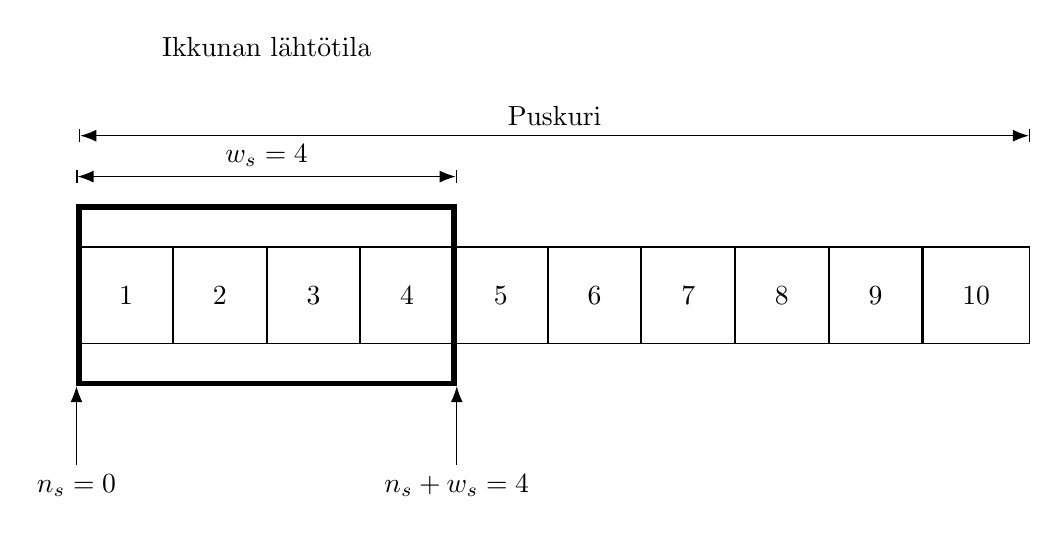
\begin{tikzpicture}[]
        
        \node(data1)[data]{1};
        \foreach \x [remember=\x as \lastx (initially 1)] in {2,...,10}{
            \node(data\x)[data, right=0cm of data\lastx]{\x};
        };
        
        
        \node (window) [draw=black, line width=2pt, inner xsep=0, inner ysep=0.5cm, fit=(data1) (data2) (data3) (data4) ] {};
        
        \node (windowStart)[below=of window.south west]{$n_s = 0$};
        \draw [->] (windowStart) -- (window.south west);
        
        \node (windowEnd)[below=of window.south east]{$n_s + w_s = 4$};
        \draw [->] (windowEnd) -- (window.south east);
        
        \node (windowDesc) [above=5.0em of window] {Ikkunan lähtötila};

        \draw [|<->|] ([yshift=1em]window.north west) -- node[above] {$w_s = 4$} ([yshift=1em]window.north east);
       
        \draw [|<->|] ([yshift=4.0em]data1.north west) -- node[above] {Puskuri} ([yshift=4.0em]data10.north east);
        
    \end{tikzpicture}
    \\[1cm]
    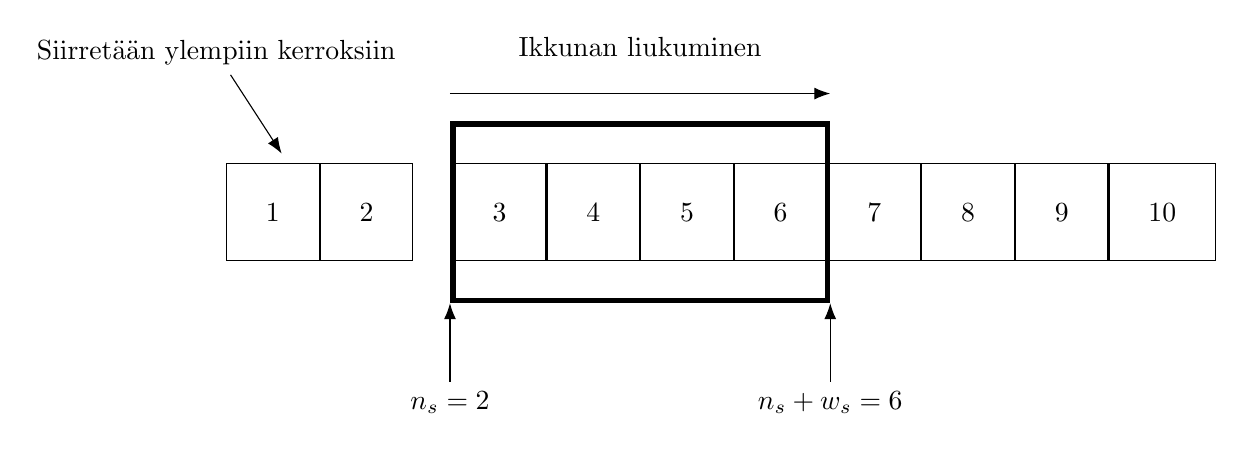
\begin{tikzpicture}[]
    
        \node(data1)[data]{1};
        \node(data2)[data, right=0cm of data1]{2};
        \node(data3)[data, right=0.5cm of data2]{3};
        \foreach \x [remember=\x as \lastx (initially 3)] in {4,...,10}{
            \node(data\x)[data, right=0cm of data\lastx]{\x};
        };

        \node (shiftedNodes) [fit=(data1) (data2)] {};

        \node (shiftDesc) [above=of shiftedNodes.north west] {Siirretään ylempiin kerroksiin};
       \draw [->] (shiftDesc) -- (shiftedNodes) {}; 
        
        \node (window) [draw=black, line width=2pt, inner xsep=0, inner ysep=0.5cm, fit=(data3) (data4) (data5) (data6) ] {};
        
        
        \node (windowDesc) [above=2.0em of window] {Ikkunan liukuminen};

        \node (windowStart)[below=of window.south west]{$n_s = 2$};
        \draw [->] (windowStart) -- (window.south west);
        
        \node (windowEnd)[below=of window.south east]{$n_s + w_s = 6$};
        \draw [->] (windowEnd) -- (window.south east);
        
        \draw [->] ([yshift=1em]window.north west) -- ([yshift=1em]window.north east);
        
    \end{tikzpicture}
    \caption{Liukuvan ikkunan toiminta} \label{fig:sliding_window}
\end{figure}
}